\documentclass{article} % For LaTeX2e
% We will use NIPS submission format
\usepackage{nips13submit_e,times}
% for hyperlinks
\usepackage{hyperref}
\usepackage{url}
% For figures
\usepackage{graphicx}
\usepackage{subfigure}
% math packages
\usepackage{amsmath}
\usepackage{amsfonts}
\usepackage{amsopn}
\usepackage{ifthen}
\usepackage{natbib}

\title{Machine Learning Project I by Group KATHMANDU}

\author{
Jade Copet\\
EPFL \\
\texttt{jade.copet@epfl.com} \\
\And
Merlin Nimier David\\
EPFL \\
\texttt{merlin.nimier-david@epfl.com} \\
\And
Krishna Raj Sapkota\\
EPFL \\
\texttt{krishna.sapkota@epfl.com} \\
}

\nipsfinalcopy

\begin{document}
\maketitle



\begin{abstract}
  In this report, we summarize our findings for the project-I. We analyzed two datasets, regression (D1) and classification (D2).
\end{abstract}



\section{The regression dataset (D1)}

  \subsection{Dataset description}
  Our training data consists of output variable $\mathbf{y}$ and input variables $\mathbf{X}$. We have $N = 1400$ data examples. Each input vector $\mathbf{x}_n$ is of dimensionality $D = 44$. Out of these 44 features, 35 are real-valued while 4 variables are binary and 5 variables are categorical, 4 of them with 4 categories and 1 with 3 categories.

  We also have test data where we do not observe $\mathbf{y}$. We have $N = 600$ test examples. Our goal is to produce predictions for test examples, as well as an approximation of the test error.

  \subsection{Data visualization and cleaning}
  We start by plotting the distribution of the input to obtain Figure \ref{fig:histY}. We notice a gaussian centered around 2500, but also a large number of data points above 6500. These points are too numereous to be discarded as outliers: we make the hypothesis that our dataset includes two models.\\

  Since inpute variables are not normalized, we center and rescale them before going forward. Plotting each input variable against the output, we notice that feature 35 seems to allow us to separate linearly the two hypothetical models. The categorical variables do not help in an obvious way, as we could have hoped. We separate points roughly at $X_{35} > 1$ (after normalization) and plot the results in Figure \ref{fig:twoModelsRough}.

  \begin{figure}[!t]
  \center
  \subfigure[Distribution of output $\mathbf{y}$. There are to many values above 6500 to discard them as outliers.]{
    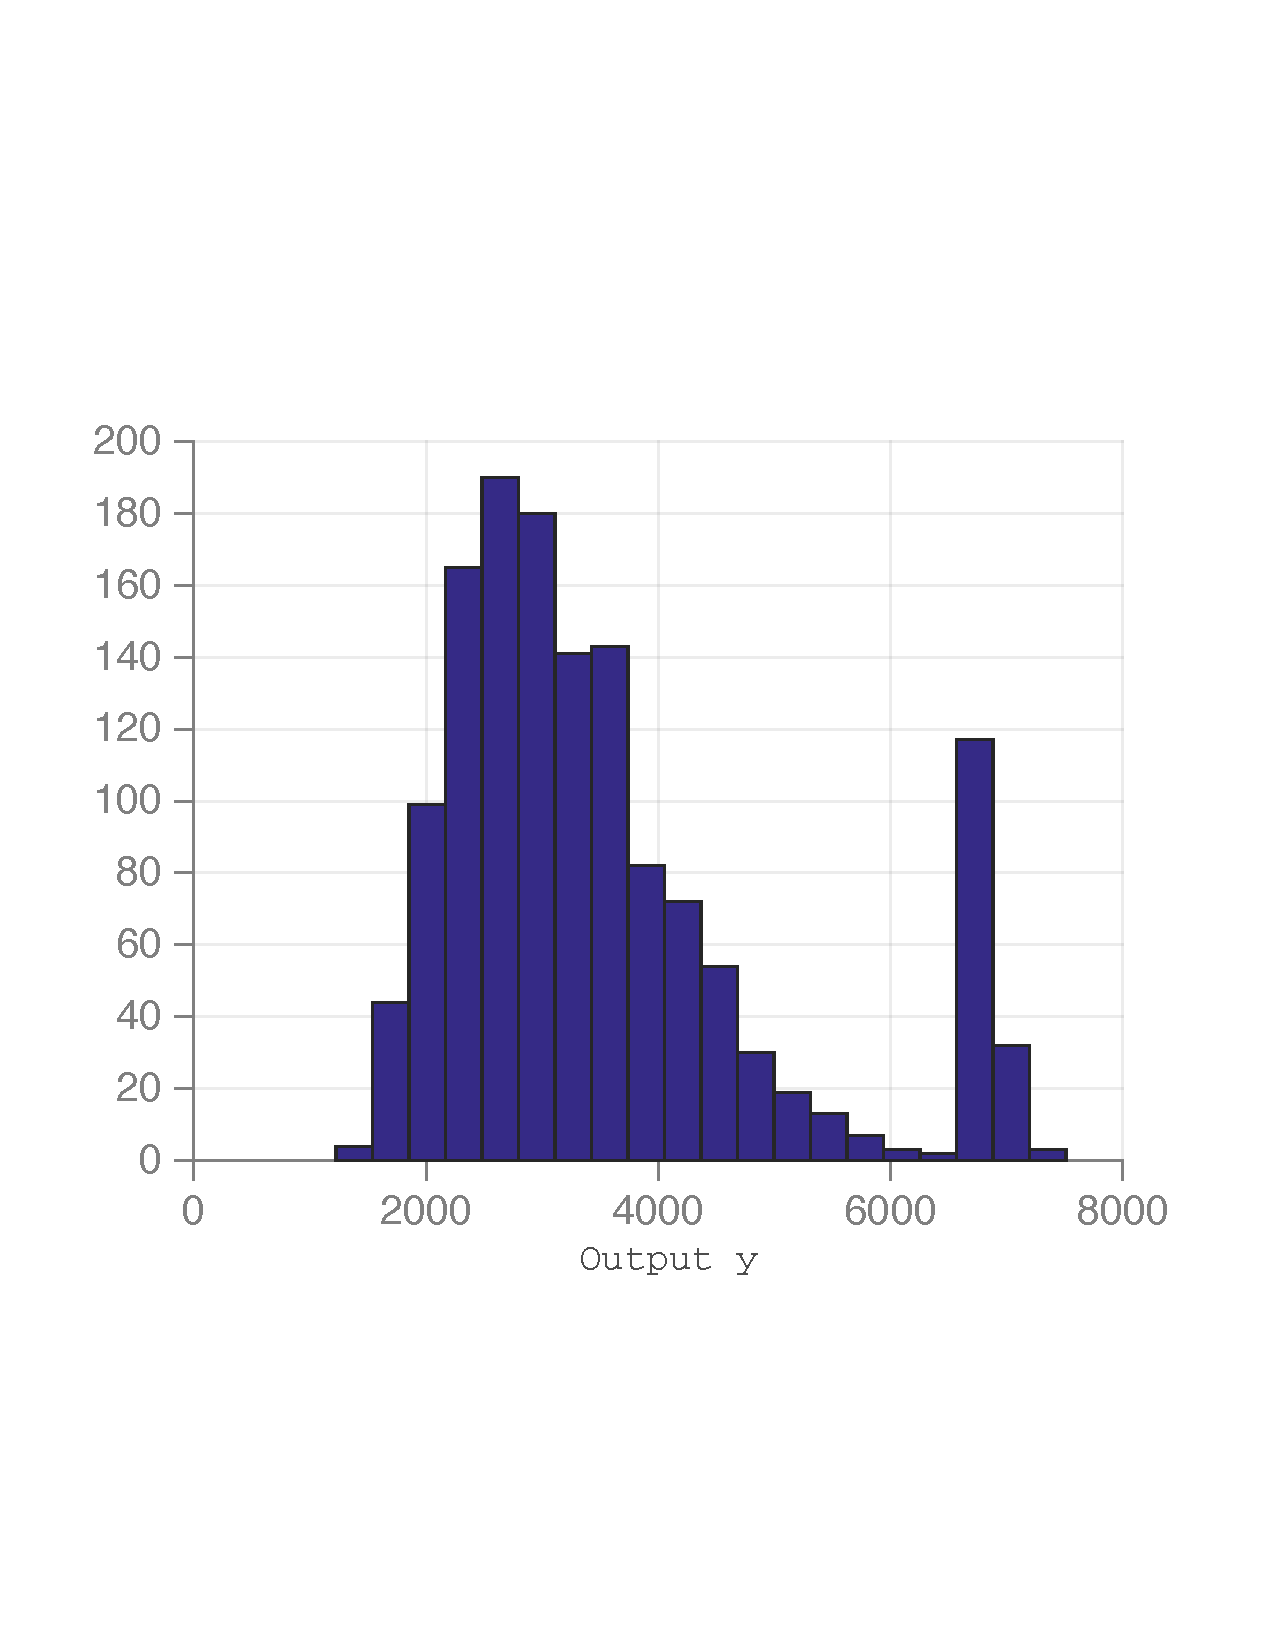
\includegraphics[width=2.5in]{figures/regression/hist-Y.pdf}
    \label{fig:histY}
  }
  \hfill
  \subfigure[$X_{35}$ seems to enable us to linearly separate the two models simply]{
    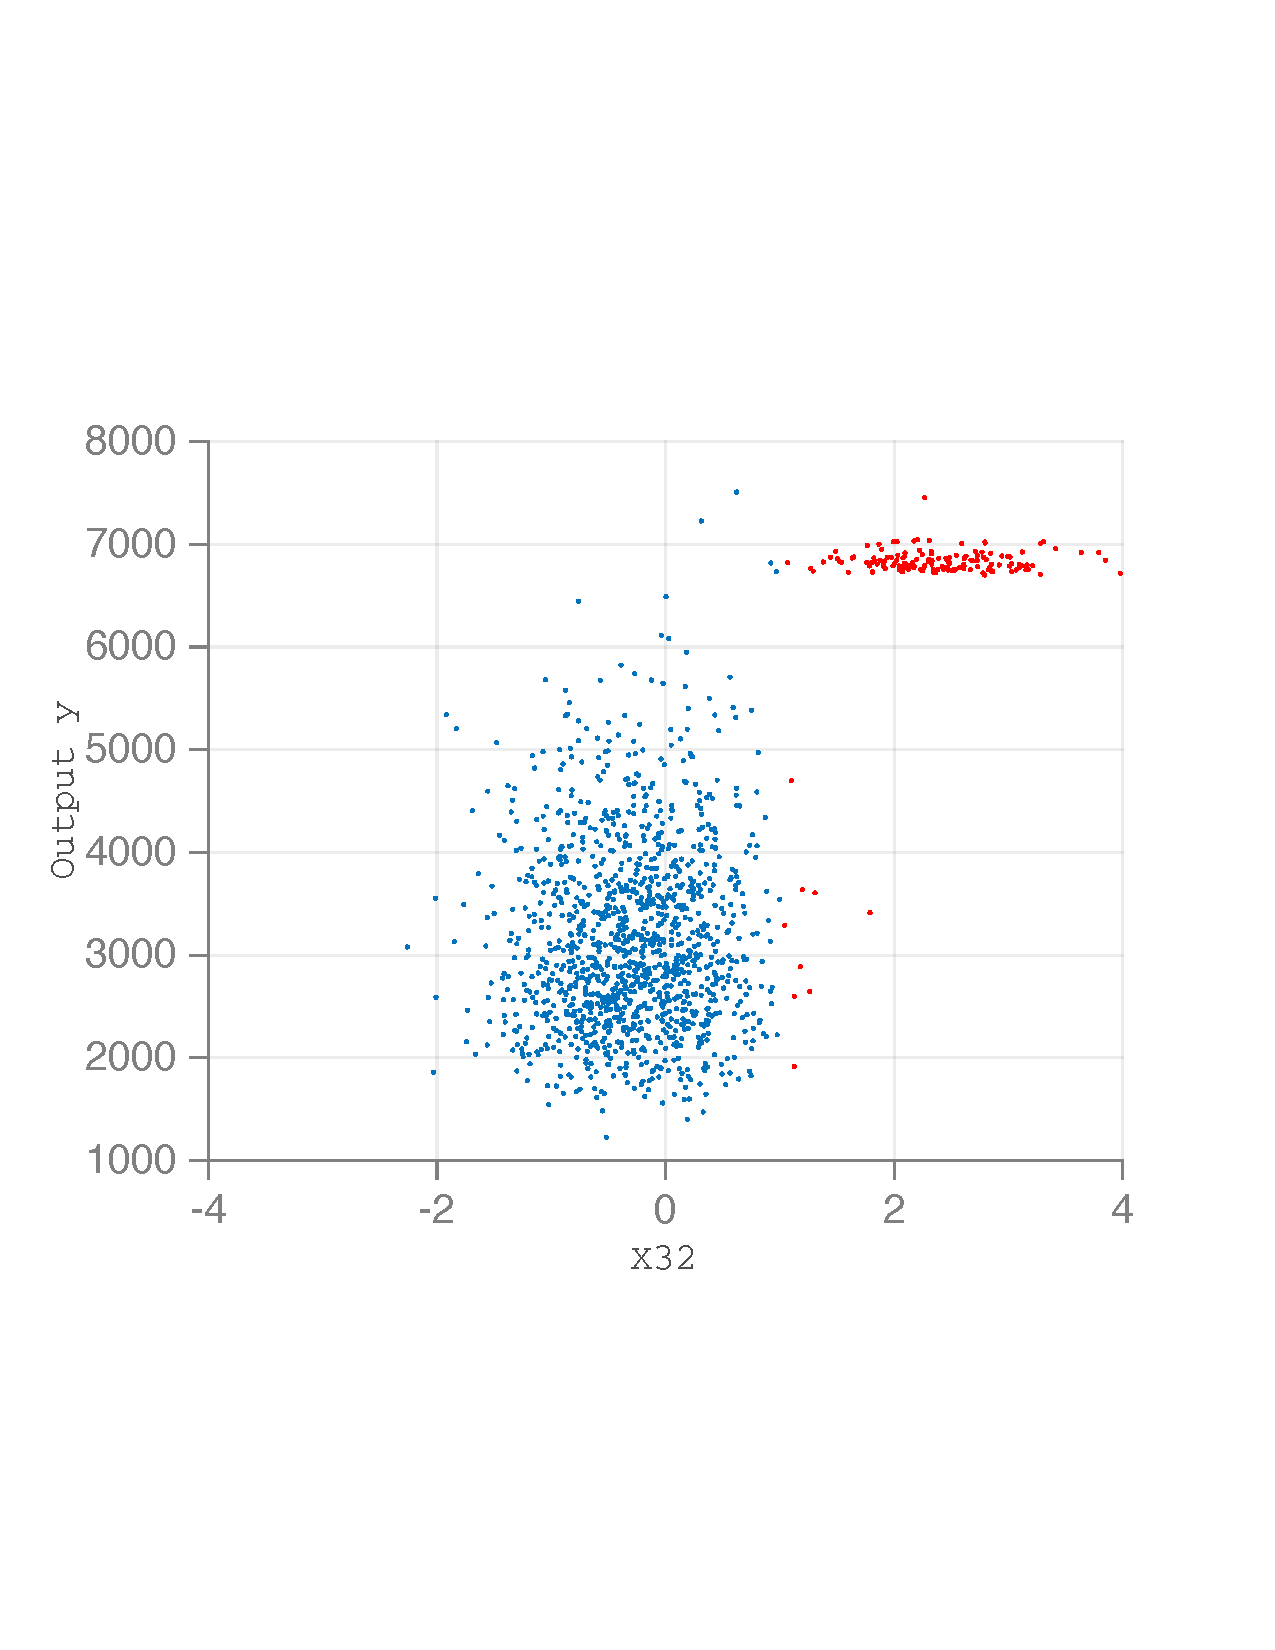
\includegraphics[width=2.5in]{figures/regression/model-separation-X35.pdf}
    \label{fig:twoModelsRough}
  }
  \hfill
  \subfigure[First try at separating the two models using $X_{35} > 1$]{
    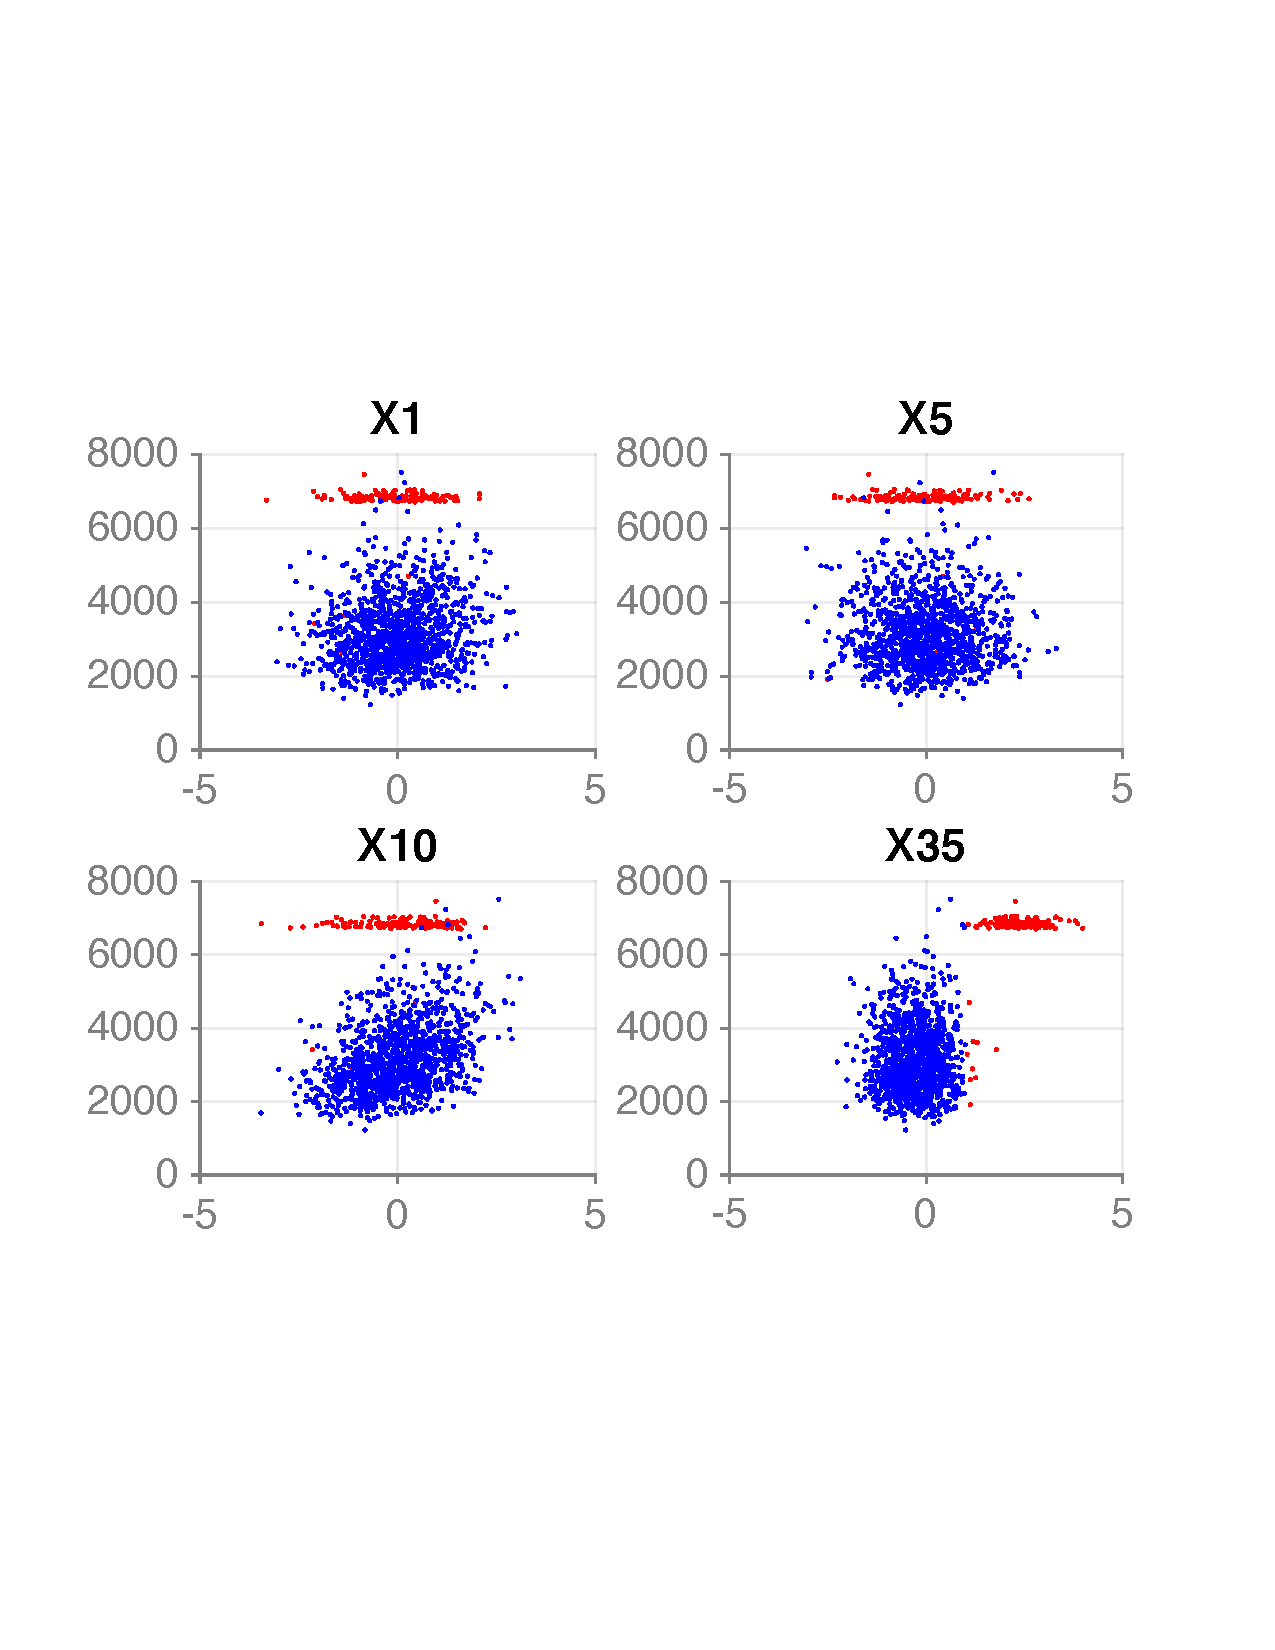
\includegraphics[width=4in]{figures/regression/model-separation-rough.pdf}
    \label{fig:twoModelsRough}
  }
  \caption{}
  \end{figure}

  - (Not rank deficient)\\
  - Correlations : results in a table ? we might be able to remove some features (go to regressionFitSelectedFeatures)\\
  - Dummy variables encoding

  \subsection{Regression fit}
  - one-variable model VS least squares VS ridge regression\\
  - RMSE errors\\
  - Discussion on overfitting, proportion selection, validation...

  \subsection{Feature transformations}
  - use ridge regression because of the resulting matrix singularity\\
  - compare different polynomial degrees (box plots, rmse values), selection and validation

  \subsection{Predictions}



\section{The classification dataset (D2)}
  We applied many of the same techniques to D2.

  \subsection{Dataset description}
  This dataset has $N = 1500$ data examples with dimensionality $D = 32$, as well as $N' = 1500$ test examples. Out of these 32 features, 29 are real-valued and 3 are categorical. Output $\mathbf{y}$ is a binary variable, which implies we are faced with a classification problem. 1052 examples belong to class $C_1$ (for which $y = 0$) and 448 examples belong to $C_2$. Like before, our goal is to produce predictions for test examples, as well as an approximation of the test error.

  \subsection{Data visualization and cleaning}

  \subsection{Regression fit}

  \subsection{Feature transformations}

  \subsection{Predictions}



\section{Summary}

\subsubsection*{Acknowledgments}

\subsubsection*{References}

\end{document}
